% ----------------------------------------------------------
% Introdução
% ----------------------------------------------------------
\chapter{Introdução}\label{cap:introducao}
%\addcontentsline{toc}{chapter}{Introdução}
% ----------------------------------------------------------

O conceito de computação em nuvem ou \textit{Cloud Computing} tem se tornado popular nos últimos anos. Seu objetivo é prover serviços de acesso a aplicações e arquivos por meio da internet de maneira flexível e simples \cite{surveycloud:2012}. A Computação em Nuvem propõe uma arquitetura diferente da cliente-servidor, na qual os recursos são diversificados e encontram-se dispersos em \textit{clusters} de sistemas distribuídos e servidores ao redor do mundo. 

A disponibilidade e o acesso a estes recursos é transparente ao usuário final e adaptável de acordo com a demanda. Neste contexto, grande parte da preocupação se concentra em atribuir as tarefas para os nós da nuvem de forma eficiente. Isto é feito para que o esforço e processamento de requisições seja feito da melhor maneira possível \cite{comparativestudy:2010}.  

Para isto, a qualidade dos serviços oferecidos de acordo com a demanda dependem, também, da arquitetura do serviço e de como é feita a virtualização dos servidores e sistemas distribuídos. Geralmente, há três diferentes tipos de serviços de computação em nuvem: armazenamento virtual, chamado \textit{Infrastructure as a Service - IaaS}, tal como Amazon Web Services \cite{amazon-cloud}; \textit{Software as a Service - SaaS}, caracterizados por provedores de serviços na internet; e, por fim, ferramentas de desenvolvimento de \textit{software} e produtos \textit{Platform as a Service - PaaS} \cite{loadbalnn}, como por exemplo a plataforma \textit{SoftLayer} \cite{softlayer2}.

Além dessa, há ainda a caracterização pelo tipo de nuvem, que podem ser públicas, privadas ou híbridas. A primeira tem como característica maior eficiência e distribuição de recursos, como por exemplo \textit{Amazon Web Services}. A segunda caracteriza-se por ser mais fechada, geralmente pertencente a uma organização específica que é responsável pelo serviço \cite{zhang2010cloud} e a última consiste em uma combinação entre as duas anteriores.

Como todas as abordagens e estruturas de serviços em nuvem precisam garantir a disponibilidade do serviço nela hospedado, há a necessidade de distribuir as requisições que chegam para os serviços de maneira eficiente, visto que a distribuição de tarefas e requisições feita de forma eficiente leva a melhora no tempo de resposta, economia de energia e diminui o risco de falhas. 

Com base nesse requisito, o balanceamento de carga tem por objetivo receber as requisições e distribuí-las para os nós do serviço de nuvem. Isto pode ser feito de diversas maneiras e a classificação dos algoritmos que realizam o balanceamento de carga é dividida, geralmente, em dois tipos: algoritmos estáticos e algoritmos dinâmicos \cite{surveycloud:2012}. Nas abordagens estáticas, as requisições são distribuídas de acordo com a capacidade do nó da nuvem de processá-la. Neste caso, é necessário ter conhecimento prévio da infraestrutura da nuvem e seus componentes. As abordagens dinâmicas, por sua vez, levam em consideração diferentes atributos dos nós, tais quais a largura de banda. Nesse caso, a distribuição é feita de forma dinâmica e requer constante monitoramento dos nós, o que geralmente torna esse tipo de balanceamento mais complexo de se implementar. 

Dentre as técnicas empregadas neste contexto é possível citar o Round-Robin, considerado um algoritmo de simples implementação, \textit{Least Connections} ou Menor Número de Conexões \cite{nginx}, \textit{Ant Colony} e até mesmo abordagens que utilizam \textit{Particle Swarm Optmization - PSO} \cite{pandey2010particle}. No entanto, sempre há maneiras de melhorar técnicas já existentes, assim como propor novas soluções.  

Com isto em mente, técnicas de reconhecimento de padrões também podem ser viáveis neste contexto. Seu objetivo é aprender uma função que melhor separe amostras de classes diferentes no espaço de características \cite{Duda:00}. Esse processo de aprendizado e reconhecimento pode ser feito por meio de Redes Neurais Artificiais (RNA) - \textit{Artificial Neural Networks (ANN)}  \cite{Haykin:07}, cuja arquitetura baseia-se na estrutura de neurônios, que por meio de redes, são capazes de realizar as mais complexas atividades. 

Tais redes podem ser representadas como grafos orientados, onde cada nó do grafo é um neurônio e o fluxo de informação é representado por suas arestas.%, como apresentado na figura 1. 
%\begin{figure}[htb]
%	\caption{\label{fig:rnn}Arquitetura simplificada de uma Rede Neural Artificial}
%	\begin{center}
%		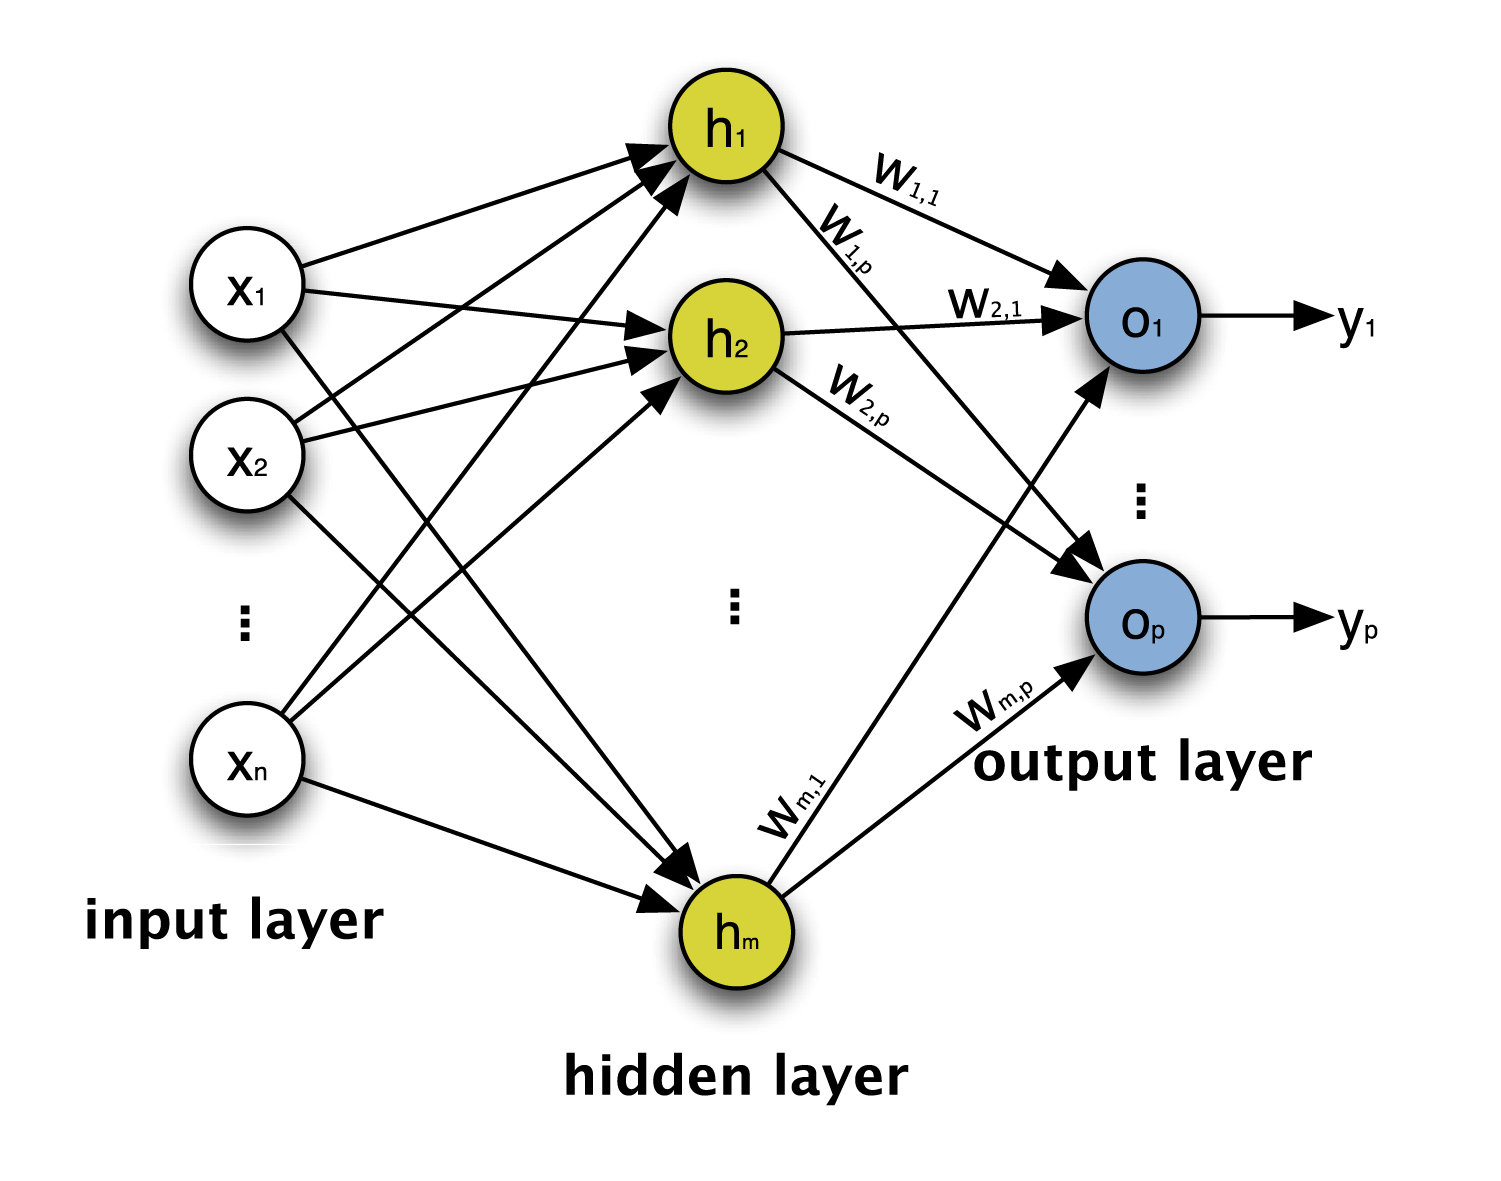
\includegraphics[width=0.5\textwidth]{img/rbf.png}
%	\end{center}
%	\legend{Fonte: elaborado pelo autor}
%\end{figure}
Os dados de entrada geralmente constituem em um vetor cujos elementos são pesos para cada uma das características da amostra.  A classificação das entradas com base no vetor de características é feito por meio de uma função de ativação sendo que cada tipo de RNA apresenta diferentes métodos de acordo com sua arquitetura. 

Dentre os vários tipos de redes neurais existentes, pode-se citar as Redes Neurais de Base Radial (\textit{Radial Basis Function - RBF}), Redes Neurais do tipo Perceptron Multi-camadas (\textit{Multilayer Perceptron - MLP}) Redes Neurais Probabilísticas (\textit{Probabilistic Neural Networks - PNNs}) \cite{specht1990} \cite{specht1992}. Por possuírem uma arquitetura mais simplista, as RBFs tem sido objeto de estudo de diversos trabalhos, bem como as PNNs e suas versões melhoradas. 

A aplicação de RNAs no contexto de balanceamento de cargas é ainda pouco explorado e pode apresentar bons resultados. Como o balanceamento de carga em sistemas de nuvem dependem, de certa forma, das características do serviço e/ou da requisição, o presente projeto propõe uma abordagem no contexto apresentado utilizando RNAs. Tendo estes conceitos em vista, o presente projeto tem por objetivo um protótipo de aplicação de RNAs no balanceamento de carga em sistemas em nuvem. 


% ---
% Objetivos
% ---
\section{Objetivos}\label{cap:objetivos-justificativa}
% ---

% ---
% Objetivos Gerais
% ---
\subsection{Objetivos Gerais}\label{sec:objetivos-gerais}
% ---

O objetivo geral deste projeto é planejar e desenvolver um módulo de aplicação que utiliza uma rede neural artificial no balanceamento de carga em serviços de nuvem, bem como analisar seu uso em ambientes reais.

% ---

% ---
\subsection{Objetivos Específicos}\label{sec:objetivos-especificos}
% ---

\begin{alineas}
	\item Estabelecer o estado da arte acerca de aplicação de redes neurais artificiais no contexto de balanceamento de carga em sistemas de nuvem;
	\item Estudar o funcionamento de serviços em nuvem;
	\item Identificar características e requisitos considerados no balanceamento de carga;
	\item Definir os elementos necessários para desenvolvimento da aplicação que fará o balanceamento;
	\item Definir tipo de RNA a ser utilizada;
	\item Planejar a estrutura da aplicação;
	\item Implementar a ferramenta inteligente;
	\item Analisar os resultados no contexto de balanceamento de carga;
\end{alineas}


\section{Organização da Monografia}

O presente trabalho divide-se em seções, sendo esta a primeira (Introdução). As demais seções estão dispostas na seguinte ordem: 
\begin{itemize}[noitemsep]
	\item \textbf{Seção 2 - Fundamentação Teórica:} apresentação dos conceitos teóricos envolvidos no trabalho. 
	\item \textbf{Seção 3 - Metodologia: } descrição do método de pesquisa e desenvolvimento, bem como as ferramentas utilizadas. 
	\item \textbf{Seção 4 - Arquitetura do Projeto:} descrição da arquitetura do projeto e da abordagem utilizada na implementação e testes. 
	\item \textbf{Seção 5 - Resultados:} apresentação dos resultados obtidos no trabalho.
	\item \textbf{Seção 6 - Conclusão:} considerações finais sobre o trabalho e possíveis trabalhos futuros.
\end{itemize}


% ---
% ----------------------------------------------------------